\documentclass[tikz]{standalone}
\usepackage{tikz}
\usetikzlibrary{positioning, graphs}
\usetikzlibrary{graphs.standard}
\usetikzlibrary{arrows.meta}
\begin{document}
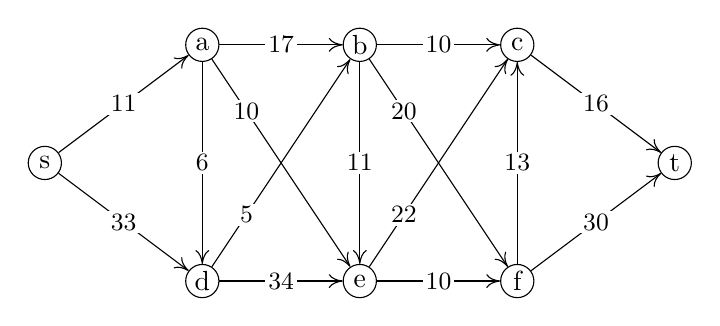
\begin{tikzpicture}
\begin{scope}
		[vertex/.style={draw,circle,inner sep = 0em, minimum size = 1.2em},
		 edgelabel/.style = {fill = white, inner sep = 0.1em, font=\small}]
		\node[vertex] (s) at (0,0) {s};
		\node[vertex] (a) at (2,1.5) {a};
		\node[vertex] (b) at (4,1.5) {b};
		\node[vertex] (c) at (6,1.5) {c};
		\node[vertex] (d) at (2,-1.5) {d};
		\node[vertex] (e) at (4,-1.5) {e};
		\node[vertex] (f) at (6,-1.5) {f};
		\node[vertex] (t) at (8,0) {t};
		
		\draw[-{>[length=5, width=5]}] (s) to node[edgelabel] {$11$} (a);
		\draw[-{>[length=5, width=5]}] (s) to node[edgelabel] {$33$} (d);
		\draw[-{>[length=5, width=5]}] (a) to node[edgelabel] {$6$} (d);
		\draw[-{>[length=5, width=5]}] (a) to node[edgelabel] {$17$} (b);
		\draw[-{>[length=5, width=5]}] (a) to node[edgelabel, near start] {$10$} (e);
		\draw[-{>[length=5, width=5]}] (d) to node[edgelabel, near start] {$5$} (b);
		\draw[-{>[length=5, width=5]}] (d) to node[edgelabel] {$34$} (e);
		\draw[-{>[length=5, width=5]}] (b) to node[edgelabel] {$10$} (c);
		\draw[-{>[length=5, width=5]}] (b) to node[edgelabel, near start] {$20$} (f);
		\draw[-{>[length=5, width=5]}] (b) to node[edgelabel] {$11$} (e);
		\draw[-{>[length=5, width=5]}] (e) to node[edgelabel, near start] {$22$} (c);
		\draw[-{>[length=5, width=5]}] (e) to node[edgelabel] {$10$} (f);
		\draw[-{>[length=5, width=5]}] (f) to node[edgelabel] {$13$} (c);
		\draw[-{>[length=5, width=5]}] (f) to node[edgelabel] {$30$} (t);
		\draw[-{>[length=5, width=5]}] (c) to node[edgelabel] {$16$} (t);
		
\end{scope}
\end{tikzpicture}
\end{document}